
\subsubsection{Reconfiguration with compensation in case of residual fault detection}

\begin{figure}
	\centering
	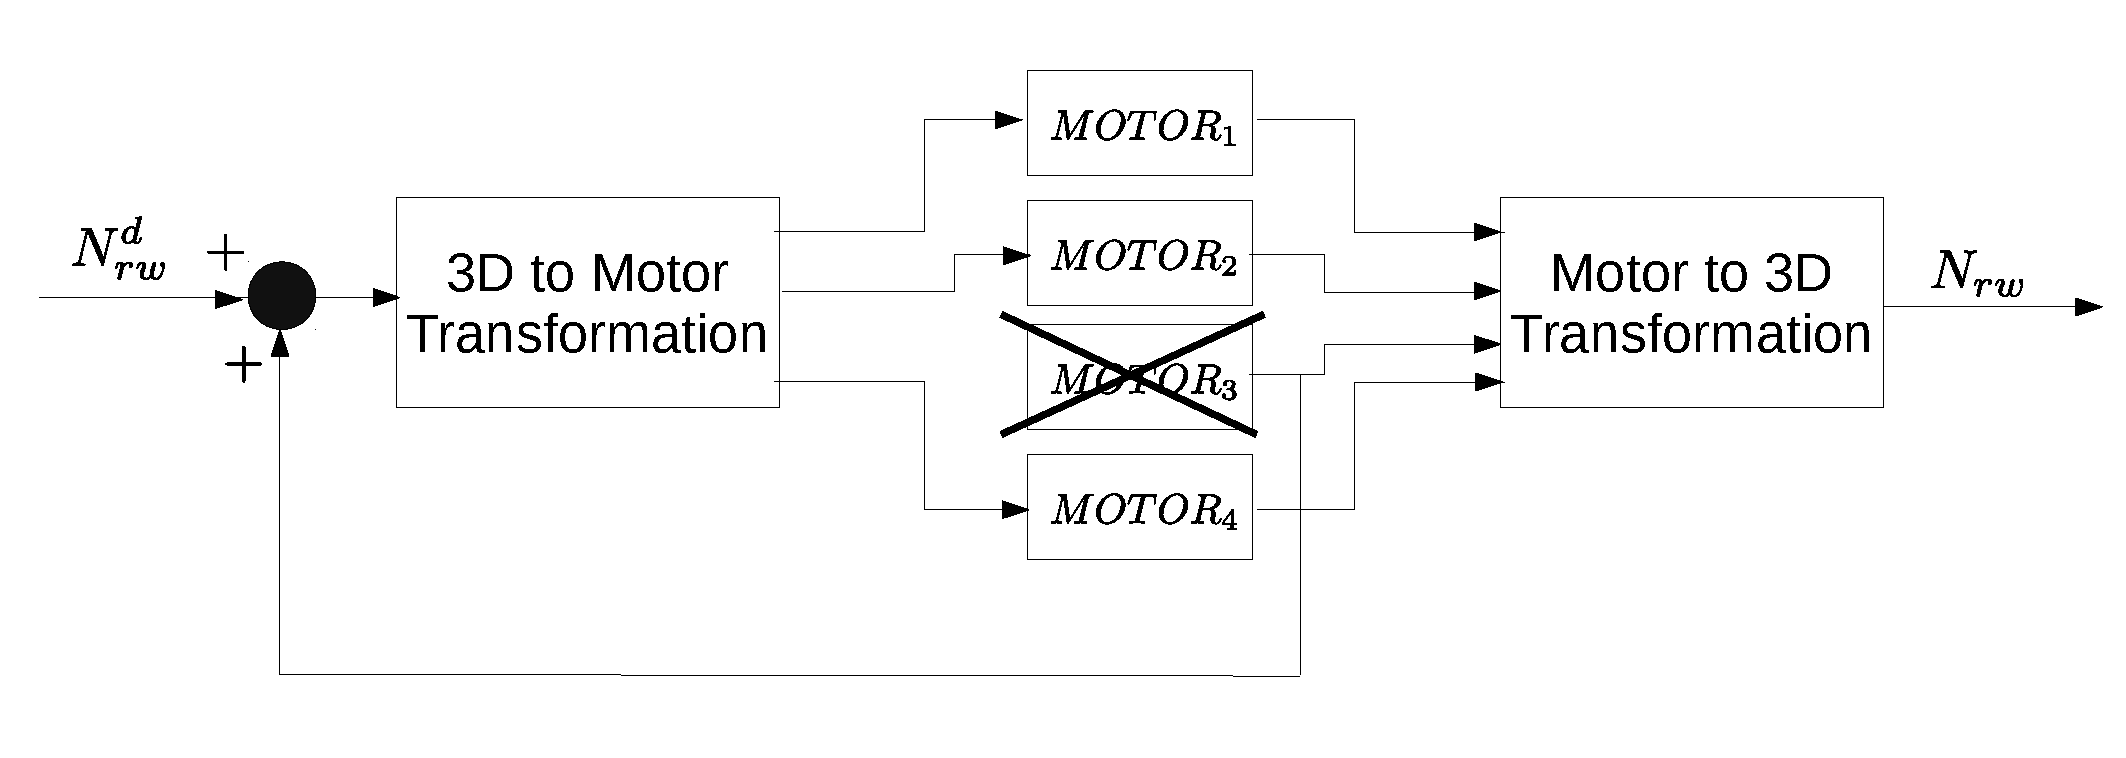
\includegraphics[width=120mm]{figures/residReconfigCompensation}
	\caption{Shutdown torque compensation in case of fault detected through residual.}
	\label{fig:angFaultCompensation}
\end{figure} 


\begin{figure}
	\centering
	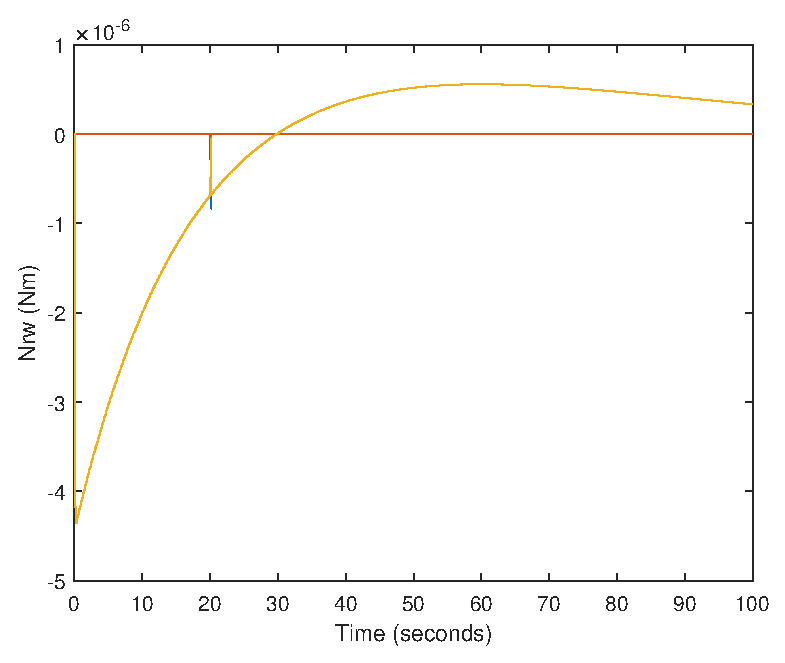
\includegraphics[width=120mm]{figures/3dTorque_resid_reconfig}
	\caption{$N_rw$ with fault occuring at 20 seconds}
\end{figure} 

\begin{figure}
	\centering
	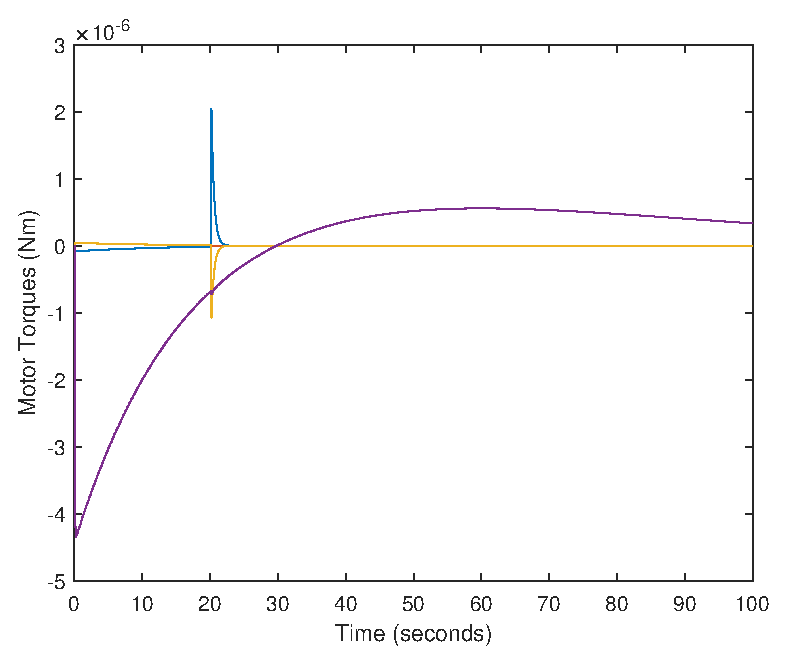
\includegraphics[width=120mm]{figures/torque_reconfig}
	\caption{$N_M$ with fault occuring at 20 seconds}
\end{figure} 

\begin{figure}
	\centering
	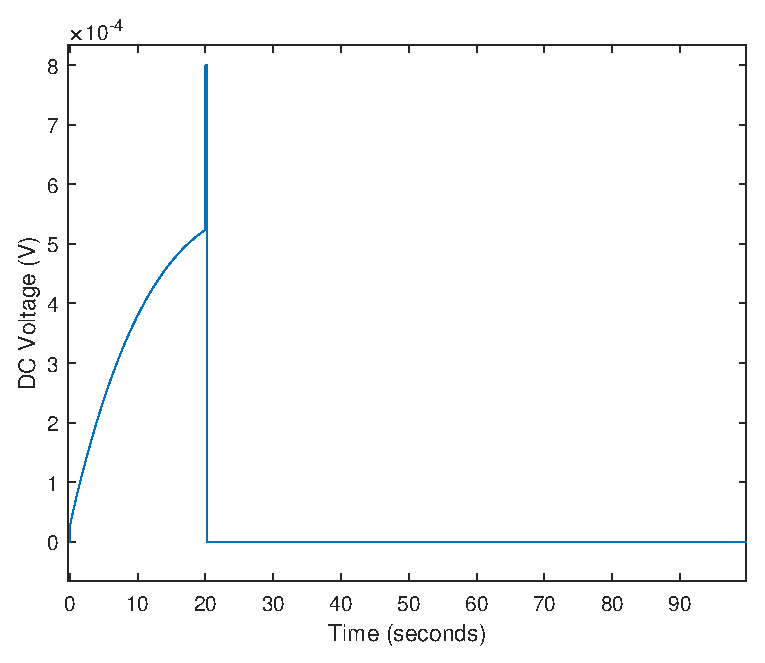
\includegraphics[width=120mm]{figures/voltage_reconfig}
	\caption{Voltage control signal with fault occuring at 20 seconds}
\end{figure} 


\begin{figure}
	\centering
	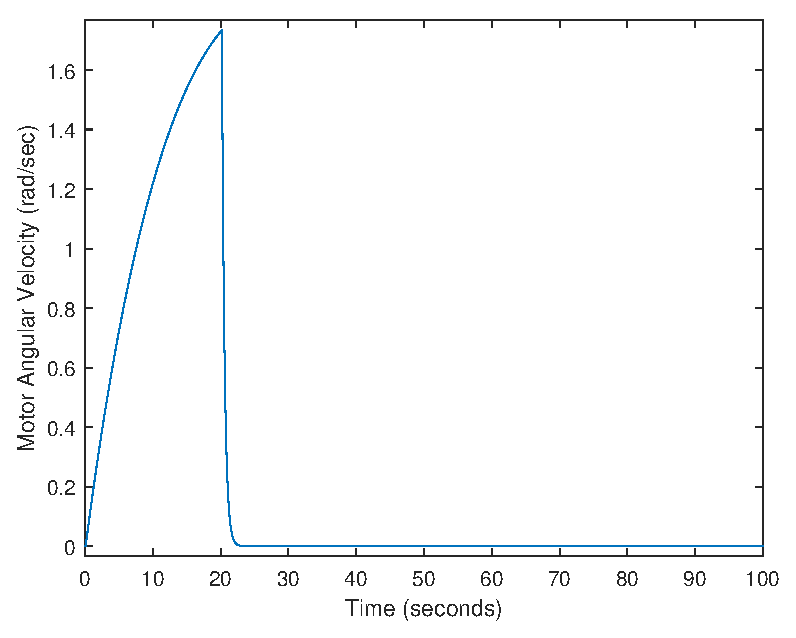
\includegraphics[width=120mm]{figures/omega_reconfig}
	\caption{$\omega_{M,i}$ with fault occuring at 20 seconds}
\end{figure} 


\begin{figure}
	\centering
	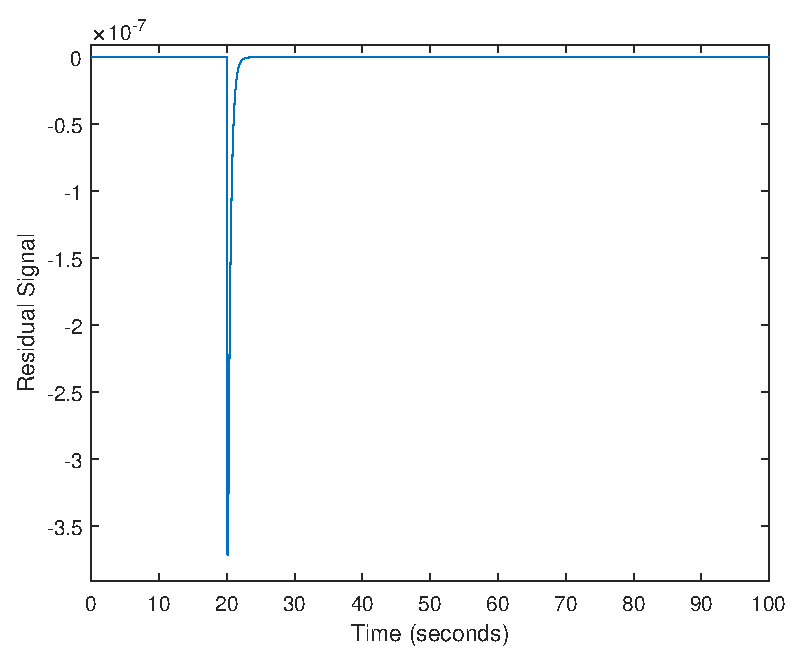
\includegraphics[width=120mm]{figures/residual_reconfig}
	\caption{Residual signal with fault occuring at 20 seconds}
\end{figure} 

\begin{figure}
	\centering
	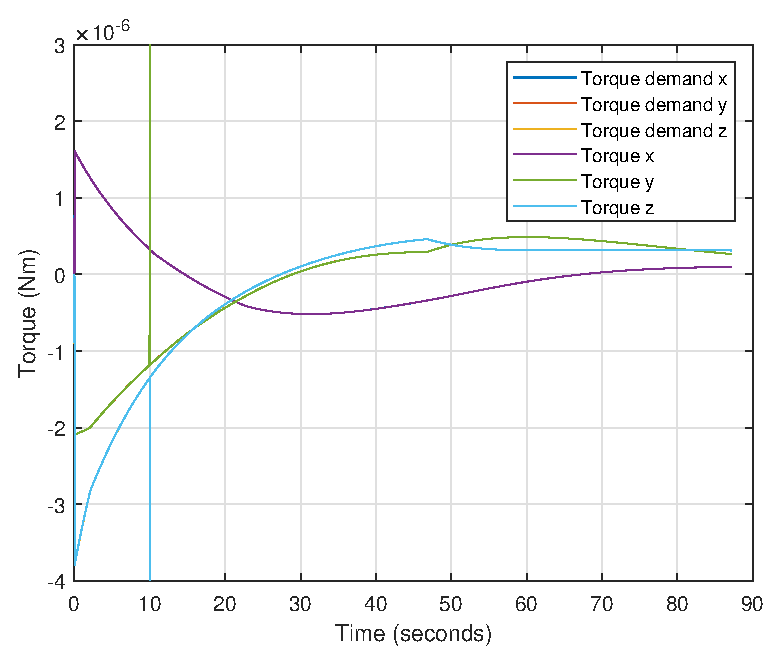
\includegraphics[width=120mm]{figures/smooth3dtorque}
	\caption{ads}
\end{figure} 

\begin{figure}
	\centering
	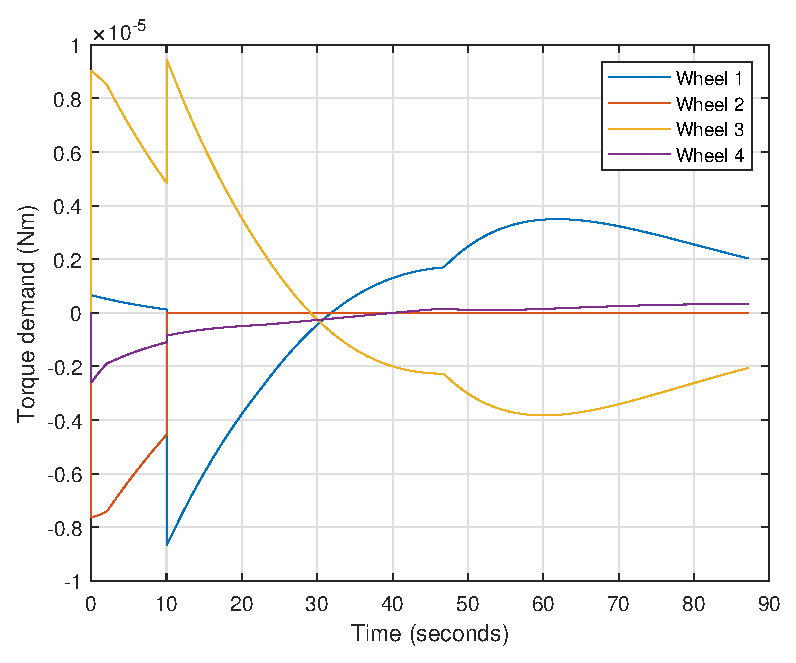
\includegraphics[width=120mm]{figures/smooth_motor_torque}
	\caption{ads}
\end{figure} 

\begin{figure}
\centering
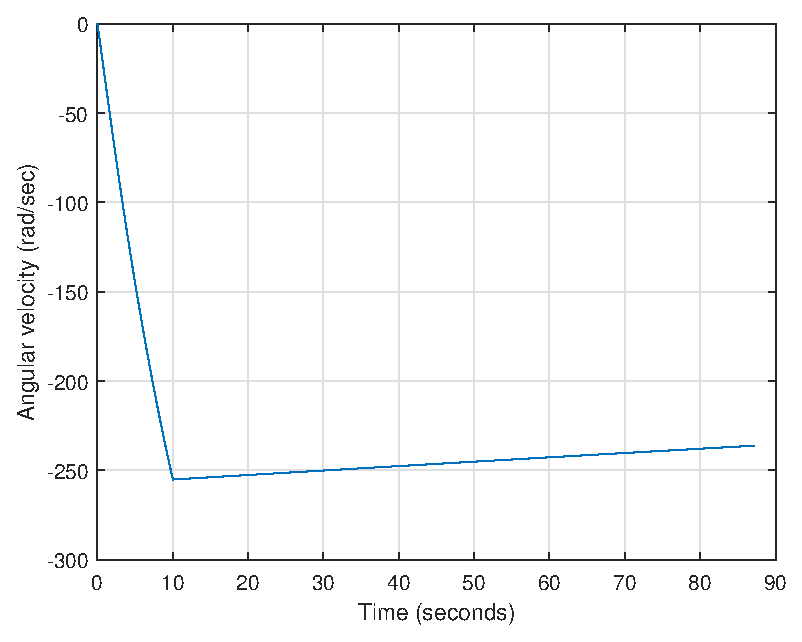
\includegraphics[width=120mm]{figures/smooth_omega_residual}
\caption{ads}
\end{figure} 